%; whizzy chapter
% -initex iniptex -latex platex -format platex -bibtex jbibtex -fmt fmt
% 以上 whizzytex を使用する場合の設定。

%     Kansai Debian Meeting resources
%     Copyright (C) 2007 Takaya Yamashita
%     Thank you for Tokyo Debian Meeting resources

%     This program is free software; you can redistribute it and/or modify
%     it under the terms of the GNU General Public License as published by
%     the Free Software Foundation; either version 2 of the License, or
%     (at your option) any later version.

%     This program is distributed in the hope that it will be useful,
%     but WITHOUT ANY WARRANTY; without even the implied warranty of
%     MERCHANTABILITY or FITNESS FOR A PARTICULAR PURPOSE.  See the
%     GNU General Public License for more details.

%     You should have received a copy of the GNU General Public License
%     along with this program; if not, write to the Free Software
%     Foundation, Inc., 51 Franklin St, Fifth Floor, Boston, MA  02110-1301 USA

%  preview (shell-command (concat "evince " (replace-regexp-in-string "tex$" "pdf"(buffer-file-name)) "&"))
% 画像ファイルを処理するためにはebbを利用してboundingboxを作成。
%(shell-command "cd image200708; ebb *.png")

%%ここからヘッダ開始。

\documentclass[mingoth,a4paper]{jsarticle}
\usepackage{kansaimonthlyreport}
\usepackage{ascmac}

% 日付を定義する、毎月変わります。
\newcommand{\debmtgyear}{2008}
\newcommand{\debmtgdate}{29}
\newcommand{\debmtgmonth}{4}
\newcommand{\debmtgnumber}{12}

\begin{document}

\begin{titlepage}

% 毎月変更する部分, 本文の末尾も修正することをわすれずに

 第\debmtgnumber{}回 関西 Debian 勉強会資料

\vspace{2cm}

\begin{center}
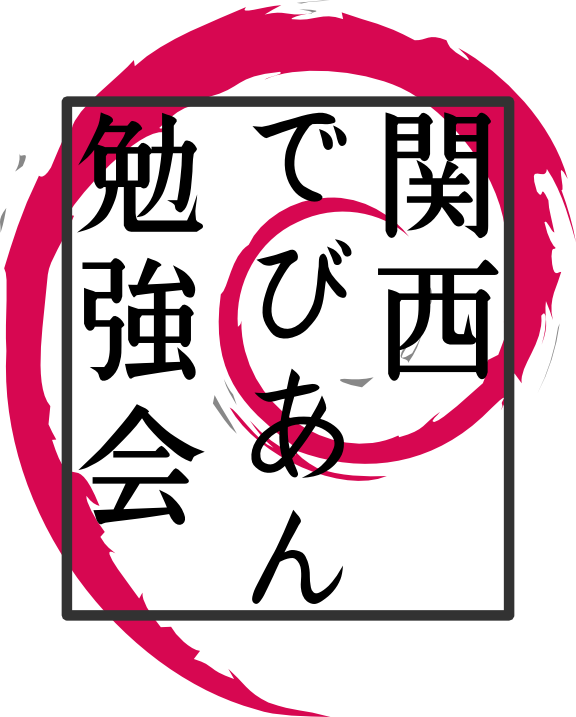
\includegraphics{image200802/kansaidebianlogo.png}
\end{center}

\begin{flushright}
\hfill{}関西 Debian 勉強会担当者 山下 尊也\\
\hfill{}\debmtgyear{}年\debmtgmonth{}月\debmtgdate{}日
\end{flushright}

\thispagestyle{empty}
\end{titlepage}

\dancersection{Introduction}{山下 尊也}
 
 関西 Debian 勉強会はDebian GNU/Linux のさまざ
 まなトピック(新しいパッケージ、Debian 特有の機能の仕組、Debian 界隈で起
 こった出来事、などなど)について話し合う会です。

 目的として次の三つを考えています。
 \begin{itemize}
  \item MLや掲示板ではなく、直接顔を合わせる事での情報交換の促進
  \item 定期的に集まれる場所
  \item 資料の作成
 \end{itemize}

 それでは、楽しい一時をお楽しみ下さい。

\newpage

\begin{minipage}[b]{0.2\hsize}
 {\rotatebox{90}{\fontsize{80}{80}
{\gt 関西デビアン勉強会}}}
\end{minipage}
\begin{minipage}[b]{0.8\hsize}
\hrule
\vspace{2mm}
\hrule
\setcounter{tocdepth}{1}
\tableofcontents
\vspace{2mm}
\hrule
\end{minipage}

\dancersection{最近のDebian関係のイベント報告}{山下 尊也}
\subsection{第11回 関西 Debian 勉強会}
2008年3月22日に「第11回 関西 Debian 勉強会」を行いました。
合計20名の参加でした。

内容は、開発よりの分野が多く、特にGPGの講座については、GPGを作るきっかけ
になったようです。

\begin{itemize}
 \item バグレポートから参加するDebianパッケージ開発 木下さん
 \item Debian 開発者のコーナーの歩き方 大浦さん
 \item GPG 最初の一歩 倉敷さん
\end{itemize}

%%% 名村さん
\dancersection{WindowsなPCでもDebianを楽しもう}{名村 知弘}
\subsection{はじめに}
Windows上でしか動かないソフトがあったり、会社のPCがWindowsだったりと、
Windowsを完全に手放すことができない環境はまだまだ多いと思います。
そんなWindowsな環境にあっても、coLinuxがあればWindowsを起動しながらにし
て、お気軽にDebianを楽しむことができます。

coLinuxの設定から、Debianを楽しむまでの流れをご紹介します。

\subsubsection{coLinuxとは何か?}
coLinux(COoperative LINUX)とは、Windows上で動作するLinuxカーネルです。
coLinux上でDebianを動作させる場合、coLinuxパッチの当てられた専用のLinux
カーネル上でDebianが動作することになります。
DebianがWindows上の1つのアプリケーションとして動作するため、Windowsを使
いながら必要になった時にDebianを起動し使用することができます。

\subsubsection{なぜcoLinuxか?}
Windows上でDebianを使う環境としては、VMWareなどのPCエミュレータが考えら
れますが、PCエミュレータはオーバヘッドやメモリ使用量が大きく、全体的に動
作が重くなってしまします。
coLinuxはWindowsアプリケーションとしてLinuxが起動するため、PCエミュレー
タに比べ動作が軽いのが特徴となっています。
ただし、ディスプレイデバイスやサウンドデバイスが実装されていないため、単
体では音のでないCUI環境となります。
\footnote{別途VNCやXサーバ、サウンドサーバを使用することで、これら機能を使用することができます。}

\subsection{coLinuxインストール}
coLinuxでDebianを使用するには、
\begin{enumerate}
\item coLinuxのインストール
\item networkの設定
\item coLinuxの設定
\end{enumerate}
の3ステップを実行します。

以下では、Windows Vista\footnote{WindowsXPでも同様の手順で作業できると思
います。}での、TAP-Win32を使用したインストールのステップを簡単に説明しま
す。


\subsubsection{coLinuxのインストール}
coLinuxの配布サイト
\footnote{\url{http://sourceforge.net/projects/colinux/files}}から、
coLinuxのインストーラ\footnote{執筆時ではkernel2.6.22をベースとした
coLinux0.7.2が最新安定版となっています}をダウンロードします。

ダウンロードしたインストーラを起動し、デフォルトのままインストールを進め
ていくと、図\ref{fig:components}のような、インストールモジュールを選択す
る画面が表示されます。
ここではネットワークアダプタとして「TAP-Win32」を使用しますので、「SLiRP」
「WinPcap」のチェックを外してください。

\begin{figure}[htbp]
 \begin{center}
  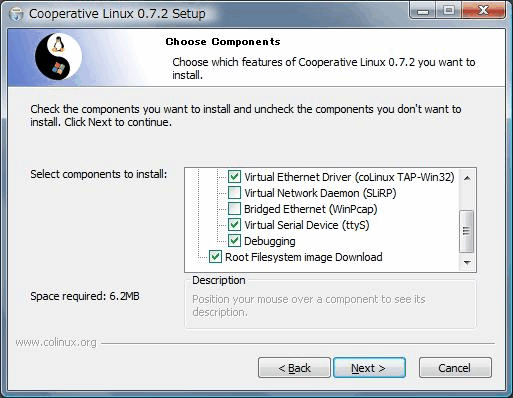
\includegraphics[width=100mm]{image200804/colinux_components.png}
 \end{center}
 \caption{インストールコンポーネントの選択}
 \label{fig:components}
\end{figure}

引き続きデフォルトのままインストールを進めていくと、図
\ref{fig:rootimage}のようなrootファイルシステムを選択する画面が表示され
るので、間違えずに「Debian」を選択してください。

\begin{figure}[htbp]
 \begin{center}
  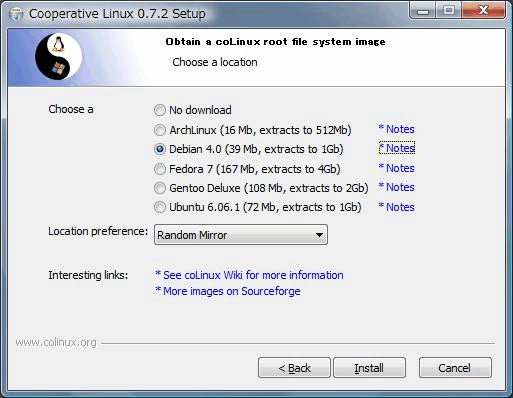
\includegraphics[width=100mm]{image200804/colinux_rootimage.png}
 \end{center}
 \caption{ルートファイルシステム選択}
 \label{fig:rootimage}
\end{figure}

あとは再びデフォルトのままインストールを進めると、インストール完了です。
ここで、「コントロールパネル」-「ネットワーク接続」を表示し、「ローカル
エリア接続 2」が作成されていると思いますので、右クリックし名前の変更を行
い、「TAP」に変更しておきます。

「ローカル エリア接続」 が2つ以上ある場合はプロパティを表示し、「接続の
方法」が「TAP-Win32 Adapter V8 (coLinux)」となっているものの名前を変更し
ます。

\subsubsection{network設定}
coLinuxの使用するネットワーク接続は、TAP-Win32(仮想ネットワークアダプタ)を使用します。
この仮想ネットワークアダプタは物理的にLANなどのネットワークに接続してい
ないため、ホストPCのReal NICを通じて物理的なネットワークに接続する必要が
あります。
物理的なネットワークに接続する方法として、ここでは以下の2つの方法をご紹介します。

Bridge接続を用いた方法

\begin{figure}[htbp]
 \begin{center}
  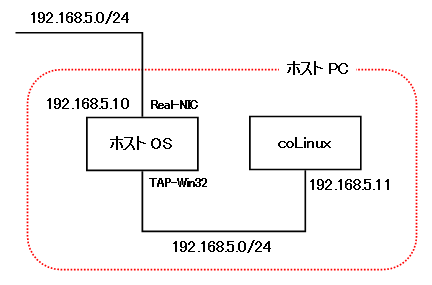
\includegraphics[width=100mm]{image200804/colinux_bridge.png}
 \end{center}
 \caption{Bridge接続を使用したネットワーク構成}
 \label{fig:bridge}
\end{figure}

Bridge接続では図\ref{fig:bridge}のように、TAP-Win32を通じてcoLinuxがReal
NICと同じサブネットに接続されるため、他のPCからもcoLinuxにアクセスするこ
とができます。
Real NICのネットワーク環境(固定IPやDHCPなど)に合わせて、coLinuxのネット
ワーク設定を行う必要があります。
長所としては、ネットワーク上の他のPCからcoLinuxに直接アクセスすることができます。
短所としては、ネットワークに接続されていない環境では、Windowsからも
coLinuxにアクセスすることができません。

設定は以下のようになります。
\begin{enumerate}
\item 「コントロールパネル」-「ネットワーク接続」を開きます。
\item 「ローカル エリア接続」と「TAP」を選択し、右クリックから「ブリッジ接続」を選択します。
\item 「ネットワークブリッジ」という接続設定が表示されたら完了です。
\end{enumerate}

ネットワーク接続の共有を用いた方法

\begin{figure}[htbp]
 \begin{center}
  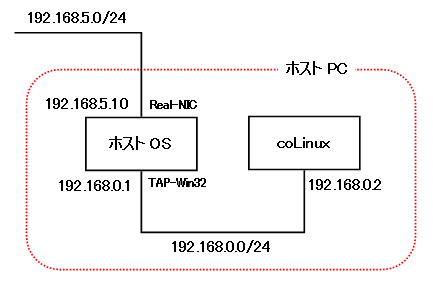
\includegraphics[width=100mm]{image200804/colinux_ics.png}
 \end{center}
 \caption{ネットワーク接続の共有を使用したネットワーク構成}
 \label{fig:ics}
\end{figure}

ネットワーク接続の共有では図\ref{fig:ics}のように、TAP-Win32はReal NICと
は異なるサブネットに参加し、ホストOSがNATになることで中継します。
TAP-Win32のIPアドレスは「192.168.0.1」固定となり、coLinuxは
「192.168.0.1/24」のIPを固定で割り当てることになります。
Real NICの接続しているサブネットが「192.168.0.0/24」の場合、IPアドレスが
バッティングしてしまうため、使用することができません。
長所としては、ネットワークに接続されていない環境でも、Windowsから常に
coLinuxに対して接続することができます。
短所としては、ネットワーク上の他のPCからはcoLinuxにアクセスすることができません。

設定は以下のようになります。
\begin{enumerate}
\item 「コントロールパネル」-「ネットワーク接続」を開きます。
\item 「ローカル エリア接続」を右クリックし、プロパティを表示します。
\item 「共有タブ」を開き、「ネットワークのほかのユーザーに、このコンピュー
      タのインターネット接続をとおしての接続を許可する」にチェックを入れ
      ます。
\item 「ホーム ネットワーク接続」は「TAP」を選択し、「OK」ボタンで閉じたら完了です。
\end{enumerate}

\begin{figure}[htbp]
 \begin{center}
  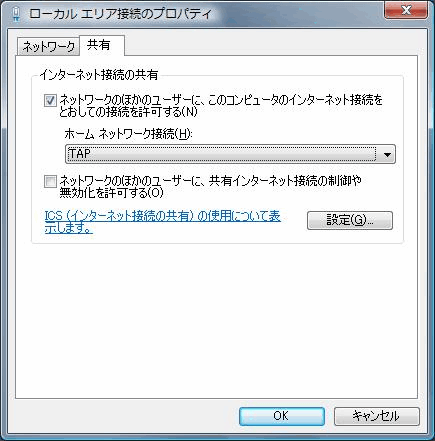
\includegraphics[width=100mm]{image200804/colinux_icssetting.png}
 \end{center}
 \caption{ネットワーク接続の共有の設定}
 \label{fig:icssetting}
\end{figure}

\subsection{coLinuxの設定}
coLinuxを起動するまでには、次の3つのステップが必要です。
\begin{itemize}
\item Debianのルートイメージの準備
\item swapディスクの準備
\item 設定ファイルの作成
\item coLinuxの起動
\end{itemize}

\subsubsection{Debianのルートイメージの準備}
coLinuxのインストール時にダウンロードされたDebianのルートイメージファイ
ルが、coLinuxインストールディレクトリに「Debian-4.0r0-etch.ext3.1gb.bz2」
というファイル名で作成されていますので、ファイルを展開\footnote{展開には、
bz2の展開ができるLhacaなどのツールが別途必要になります。}します。

展開すると「Debian-4.0r0-etch.ext3.1gb」というファイルが生成されるため、
分かりやすいように「fs-root-etch.img」などと名前を変更しておきます。

\subsubsection{swapディスクの準備}
coLinuxのインストールでは、swapファイルは用意されていないため、各自で用意する必要があります。
ここでは既に作成されたswapファイルをダウンロードできるサイトを利用してダウンロードします。

\url{http://gniarf.nerim.net/colinux/swap/}にアクセスし、「swap\_512Mb.bz2」をダウンロードします。

「swap\_512Mb.bz2」を展開すると、「swap\_512Mb」というファイルが生成され
るため、分かりやすいように「fs-swap-512.img」などと名前を変更しておきま
す。

\subsubsection{設定ファイルの作成}
これで必要なファイルは全てそろったので、coLinuxでDebianを起動するための設定を行います。

設定ファイルのフォーマットには、xmlを使用した方法と、独自のconfファイル
の2種類がありますが、ここではconfファイルを使用した方法を記載します。

coLinuxインストールディレクトリに「etch.conf」というファイルを作成し、以下の内容を記載します。

\begin{commandline}
kernel=vmlinux
initrd=initrd.gz
mem=512
#「c:\coLinux」は適宜coLinuxのインストールディレクトリで読み替えてください。
cobd0="c:\coLinux\fs-root-etch.img"
cobd1="c:\coLinux\fs-swap-512.img"
eth1=tuntap
root=/dev/cobd0
ro
\end{commandline}

coLinuxをインストールしたディレクトリに、「example.conf」というファイル
がありますので、必要であればこのファイルを参考に設定を変更してください。

\subsubsection{coLinuxの起動}
coLinuxには2通りの起動方法が用意されています。
\begin{itemize}
\item コンソールアプリケーションとして起動
\item サービスアプリケーションとして起動
\end{itemize}

以下にそれぞれの起動方法を記載します。

コンソールアプリケーションとして起動する方法\\
coLinuxのインストールディレクトリに、「colinux-daemon.exe」のショートカッ
トを作成し、プロパティから「リンク先」の末尾に「-t nt @etch.conf」を追加
します。

\begin{figure}[htbp]
 \begin{center}
  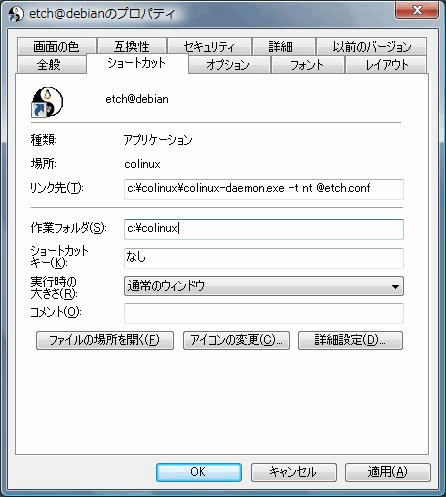
\includegraphics[width=100mm]{image200804/colinux_shortcut.png}
 \end{center}
 \caption{coLinux起動ショートカット}
 \label{fig:shortcut}
\end{figure}

このショートカットを起動すると、coLinuxがコンソールアプリケーションとして起動します。
コンソールアプリケーションとして起動しているため、コンソールを終了すると
当然coLinuxも終了してしまいます。

うっかり終了してしまうことを防ぐため、coLinuxをサービスアプリケーション
として起動する方法が用意されています。

サービスアプリケーションとして起動する方法\\
コマンドプロンプトを起動し、coLinuxのインストールディレクトリに移動し、
以下のコマンドを実行します。
「\verb|c:\coLinux|」は適宜coLinuxのインストールディレクトリで読み替えてください。
\begin{commandline}
colinux-daemon.exe "@c:\coLinux\etch.conf" --install-service
\end{commandline}

これでcoLinuxがサービスとして登録されました。ファイル名を指定して実行よ
り以下のコマンドを実行し、「Cooperative Linux」が登録されていることを確
認してください。
\begin{commandline}
%SystemRoot%\system32\services.msc
\end{commandline}

「スタートアップの種類」を「手動」に設定し、以下のコマンドでそれぞれ起動、
停止することができます。
\begin{commandline}
net start "Cooperative Linux"
net stop "Cooperative Linux"
\end{commandline}

%%% 大浦さん
\dancersection{Debian GNU/kFreeBSD}{大浦 真}

\subsection{Debian GNU/kFreeBSD とは}

Debian は、カーネルとして Linux だけをターゲットとしているのではない。
Debian GNU/kFreeBSD は、カーネルとして FreeBSD のカーネルを利用し、
その上に GNU C library と Debian のパッケージセットを移植したものである。
(カーネルだけを使っているので、``\textbf{k}FreeBSD'')

正式なリリースはまだだが、今回はそのインストール方法を紹介する。

\subsection{Debian GNU/kFreeBSD のインストール}

QEMU 上の仮想マシンにインストールする。

\begin{enumerate}
\item \url{http://glibc-bsd.alioth.debian.org/install-cd/}より
  インストール CD のダウンロード。
  現時点での最新版は、20080218 の日付のもの。
  \texttt{debian-20080218-kfreebsd-i386-install.iso}
  \begin{itemize}
  \item インストーラは、FreeBSD のインストーラを改造したものである。
    他のアーキテクチャで使われている Debian Installer は移植されていない。
  \end{itemize}
\item qemu 用のイメージの作成

  \$ \verb|qemu-img create -f qcow2 kfreebsd.img 10G|
\item qemu 起動

  \$ \verb|qemu -hda kfreebsd.img \| \\
  \verb|-cdrom debian-20080218-kfreebsd-i386-install.iso -m 512 -boot d|
\item FreeBSD のインストーラが起動したら Express を選択。
\item ハードディスクの設定。
  \begin{itemize}
  \item FDISK Partition Editor で slice の設定。
    Create Slice でハードディスク全体を選択。
  \item Boot Manager の設定。GRUB も使えるようだが、
    手動で設定する必要があるので、FreeBSD の Boot Magager を使う。
  \item FreeBSD Disklabel Editor。Partition の設定。
    ひとまず Swap Partition と / を作成。
  \end{itemize}
\item ベースシステムのインストール
  \begin{itemize}
  \item Choose Distribution で Minimal を選択。
  \item Choose Installation Media で CD/DVD を選択。
  \item CD から base system のインストールが始まる。
  \item Alt-F3 でコンソールに移る。
  \item tzdata の設定。
  \item popularity-contest の設定。
  \end{itemize}
\item インストールの終了と再起動。
  \begin{itemize}
  \item User Configuration Requested で No を選択。
  \item sysinstall Main menu に戻ったら Exit Install でインストーラを終了。
  \item 再起動。
  \end{itemize}
\item 再起動後の設定
  \begin{itemize}
  \item ユーザとしては、root のみが作成されている。
    パスワードなし。
  \item ネットワークの設定はなされていない。
    DHCP 環境の場合、dhclient を実行するとネットワークにつながる。
  \item ftp.debian-ports.org のアーカイブキーを取得。

    \$ \verb+wget -O - http://ftp.debian-ports.org/archive/archive_2008.key \+ \\
    \verb+| apt-key add -+
  \end{itemize}
\end{enumerate}

\subsection{問題点と今後}

\begin{itemize}
\item インストーラが行う設定が必要最低限のみ。
  一般ユーザの作成やネットワークの設定は自分で行う必要がある。
\item 基本的なパッケージでも移植できていないパッケージや
  きちんと動作しないパッケージが結構多い。
  (Debian GNU/Linux であることを前提して作られたパッケージが、
  GNU/kFreeBSD に持ってくるとビルドできないことがある。)
  \begin{itemize}
  \item console-tools、sysklogd、emacs22 など
  \item 現時点で、
    Architecuture: any のパッケージの 80\% ほどしかビルドできていない。

    \url{http://buildd.debian-ports.org/stats/}
  \end{itemize}
\item ハックのしがいあり。
  \begin{itemize}
  \item \url{http://glibc-bsd.alioth.debian.org/TODO}
  \item \url{http://glibc-bsd.alioth.debian.org/porting/PORTING}
  \end{itemize}
\end{itemize}

\subsection{関連リンク}

\begin{itemize}
\item \url{http://www.debian.org/ports/kfreebsd-gnu/}
\item \url{http://wiki.debian.org/Debian_GNU/kFreeBSD}
\item \url{http://glibc-bsd.alioth.debian.org/doc/} \\
  「Installing Debian GNU/kFreeBSD」
\item \url{http://tokyodebian.alioth.debian.org/html/debianmeetingresume200708se7.html} \\
  「Debian GNU/kFreeBSD のインストール」(第31回東京エリア Debian 勉強会資料)
\end{itemize}

%%% たかや
\dancersection{chrootからはじめる sid}{山下 尊也}

sid って危険って言うけど、本当に危険なんですか?とか、unstableって名前が
怖かったりとか、はたまた、本日締切りの原稿とかあるのに、新しいバージョン
なものを触ってみたいとか、いろいろあると思います。

今回は、初めてsidの環境を触ろうと考えていらっしゃる方にお勧めなものを紹介します。

debootstrapを用いれば、chrootしたDebian環境を安易に構築する事が可能です。

今回は、/home/tommy/chroot/sid の下にchroot環境なsidを構築します。

\begin{commandline}
 $ sudo mkdir -p /home/tommy/chroot/sid
 $ sudo debootstrap sid /home/tommy/chroot/sid http://ftp.jp.debian.org/debian
I: Retrieving Release
I: Retrieving Packages
I: Validating Packages
I: Resolving dependencies of required packages...
I: Resolving dependencies of base packages...
・・・
I: Configuring klogd...
I: Configuring tasksel-data...
I: Configuring tasksel...
I: Base system installed successfully.
\end{commandline}

さっそく、作った環境にログインしてみましょう。

\begin{commandline}
 $ sudo chroot /home/tommy/chroot/sid /bin/bash
root@hoge:/# 
\end{commandline}

これでログイン出来ました。

基本的なパッケージしか入っていないため、/etc/apt/souces.list を更新し、
自分に必要なパッケージなどをいれましょう。

\begin{commandline}
root@hoge:/# vi /etc/apt/sources.list
\end{commandline}

/homeなどを共有したい場合は、以下のように親の/etc/fstabに書き加えます。

\begin{commandline}
 $ sudo vi /etc/fstab
/home           /home/tommy/chroot/sid/home        none    bind            0       0
/tmp            /home/tommy/chroot/sid/tmp         none    bind            0       0 
proc-chroot     /home/tommy/chroot/sid/proc        proc    defaults        0       0 
devpts-chroot   /home/tommy/chroot/sid/dev/pts     devpts  defaults        0       0 
\end{commandline}

ユーザ情報をコピーしましょう。

\begin{commandline}
 $ sudo cp /etc/passwd /home/tommy/chroot/sid/etc/
 $ sudo sed 's/\([^:]*\):[^:]*:/\1:*:/' /etc/shadow | sudo tee /home/tommy/chroot/sid/etc/shadow
 $ sudo cp /etc/group /home/tommy/chroot/sid/etc/
 $ sudo cp /etc/hosts /home/tommy/chroot/sid/etc/
\end{commandline}

chrootは、管理者権限がなければ使う事が出来ません。
dchrootは、chrootの環境のコマンドを一般ユーザの権限で実行する事を可能に
します。アプリケーションを用いたい場合などは、一般ユーザ権限で実行したい
場合が多いと思います。

\begin{commandline}
 $ echo ``mychroot /home/tommy/chroot/sid'' | sudo tee /etc/dchroot.conf
 $ dchroot -c mychroot (ログイン)
\end{commandline}

現在、experimentalな環境に iceweaselのバージョン3ベータがきています。
これを実行する事を考えてみましょう。
まず、experimentalな環境をインストール出来るように
/etc/apt/sources.listを編集します。

\begin{commandline}
 $ dchroot -c mychroot
 $ su -
root@hoge:/# vi /etc/apt/sources.list
deb http://cdn.debian.or.jp/debian/ sid main contrib non-free
deb http://cdn.debian.or.jp/debian/ experimental main contrib non-free
\end{commandline}

そして、experimentalなIceweaselをインストールします。

\begin{commandline}
root@hoge:/# aptitude install iceweasel/experimental
\end{commandline}

dchrootは、chroot環境以下に対して、一般ユーザの権限でコマンドを用いる事
も可能です。

\begin{commandline}
 $ dchroot -c mychroot -d iceweasel
\end{commandline}

これで、chroot環境内に構築しました experimental の Iceweasel を使う事が
出来ます。

chrootは現在動いているカーネル上に仮想OSを作成することから、
オーバーヘッドが比較的小さい事が大きな利点であると思います。

すでに安定版の Debian を使っているのであれば、chrootを用いれば、
簡単に不安定版の Debian のアプリケーションを利用する事が出きるので、
ちょっと触れてみたい方にはお勧めな方法の一つだと思うので是非試してみて下
さい。

\subsection{参考文献}

\begin{itemize}
\item \url{https://wiki.ubuntulinux.jp/UbuntuPackagingGuideJa/appendix-chroot} \\ The Ubuntu Packaging Guide 日本語版/chroot環境
\item Debian辞典 著者 武藤健志
\item \url{http://kmuto.jp/d/index.cgi/debian/debootstrap.htm} \\ KeN's
      GNU/Linux Diary Etch/Sidの上にSarge環境を作る方法
\end{itemize}

\dancersection{今後の予定}{山下 尊也}

\subsection{次回}
次回は、2008年5月18日に福島区民センター
\footnote{\url{http://www.city.osaka.jp/shimin/shisetu/01/fukushima.html}}
にて行なう予定です。

\subsection{OSC 2008 Kansaiについて}
今年のOSC Kansaiの日程が決まりました。
7月18,19日(金・土)に行なわれます。

関西 Debian 勉強会として決まっているのは、
以下の通りです。

\begin{itemize}
 \item 18日に参加出来る方が多ければ、18日,19日両日参加する
 \item セッション時間は、2時間頂き、通常とほぼ同様の勉強会を開催する
 \item ブース担当と、セッション担当に分ける
\end{itemize}

\subsection{KDRのおしらせ}
関西Debian勉強会の有志で
関西Debian勉強会とは独立した形で、
週に一度、読書会(KDR)を開いています。
詳しくはKDR公開用ページ\footnote{\url{http://qwik.jp/kdrweb/}}をご覧下さ
い。

% \dancersection{メモ}{}
% \mbox{}\newpage
 
\printindex
 \cleartooddpage

 \begin{minipage}[b]{0.2\hsize}
  \rotatebox{90}{\fontsize{80}{80} {\gt 関西デビアン勉強会} }
 \end{minipage}
 \begin{minipage}[b]{0.8\hsize}

 \vspace*{15cm}
 \rule{\hsize}{1mm}
 \vspace{2mm}
 
\includegraphics[width=2cm]{image200502/openlogo-nd.eps}
 \noindent \Large \bf Debian 勉強会資料\\ \\
 \noindent \normalfont \debmtgyear{}年\debmtgmonth{}月\debmtgdate{}日 \hspace{5mm}  初版第1刷発行\\
 \noindent \normalfont 関西 Debian 勉強会 (編集・印刷・発行)\\
 \rule{\hsize}{1mm}
 \end{minipage}

\end{document}
